\chapter{Desenvolvimento da Aplicação}

Neste capítulo descrevemos os conceitos, análises e ferramentas
utilizadas pela equipe TGT para o desenvolvimento do porduto Lixt,
incluindo os requisitos do projeto, as tecnologias utilizadas, e a
arquitetura e a modelagem do produto.
Isto é apresentado para que se possa estabelecer parâmetros e métricas
que guiarão o desenvolvimento e a entrega final do projeto.

\section{Arquitetura}
Com base na análise do projeto, e nos requisitos que foram levantados
como necessários, a arquitetura cliente-servidor é plausível como
modelo para o produto que pretendemos entregar.
Esta arquitetura é composta por duas aplicações distintas:
\begin{itemize}
\item Uma aplicação \emph{front-end}, focada na interação com o usúario
  e apresentação de dados de uma forma agradável e intuitiva. Esta
  aplicação será implementada em JavaScript, com o framework React
  Native, e disponibilizada para as plataformas iOS e Android.
\item Uma aplicação \emph{back-end}, que será responsável por tratar os
  dados coletados no \emph{front-end} e disponibilizar as informações
  que serão mostradas aos usuários. Como esta aplicação requer uma
  lógica de servidor, estabilidade e ampla disponiblidade, esta
  aplicação será implementada em Java, com uso do framework Spring
  Boot, que abstrai a criação de um servidor.
\end{itemize}
Podemos ver na \autoref{fig:cli-srv} uma respresentação desta
arquitetura.

\begin{figure}
  \centering
  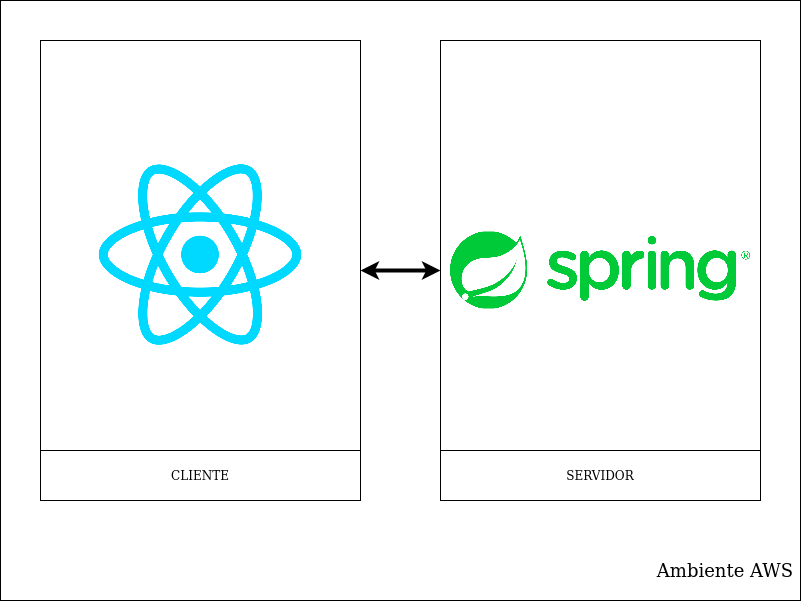
\includegraphics[scale=0.5]{lixt}
  \caption{Arquitetura Lixt}
  \label{fig:cli-srv}
\end{figure}

A comunicação entre estes serviços será feita com o uso do protocolo
\label{sig:https}\hyperlink{s:http}{HTTPS}, que permite a aplicação
cliente realizar chamadas ao servidor através de urls, seja para
buscar informações para apresentar ao usuário ou postar informações
coletadas dele. O framework Spring, além de abstrair a implementação
da lógica de um servidor, implementa \emph{listeners} para estas urls,
auxiliando a criação de pontos na aplicação do servidor focados na
comunicação com a aplicação cliente.



%%% Local Variables:
%%% mode: latex
%%% TeX-master: "../desenho"
%%% End:
